\newif\ifstandardreport
\IfFileExists{tietreport.cls}{%
  \documentclass{tietreport}
}{%
  \documentclass[11pt,a4paper]{report}
  \standardreporttrue
}

\ifstandardreport
  \usepackage[margin=25mm]{geometry}
  \newcommand{\TitlePageHeader}[1]{\def\reportheader{#1}}
  \newcommand{\ProjectTitle}[1]{\def\reporttitle{#1}}
  \newcommand{\ProjectSubTitle}[1]{\def\reportsubtitle{#1}}
  \newcommand{\TitlePageSubText}[1]{\def\reportsubtext{#1}}
  \newcommand{\AdvisorName}[1]{\def\reportadvisor{#1}}
  \newcommand{\TitlePageFooterText}[1]{\def\reportfooter{#1}}
  \makeatletter
  \renewcommand{\maketitle}{%
    \begin{titlepage}
      \centering
      {\large\bfseries\reportheader\par}
      \vspace{2cm}
      {\Huge\bfseries\reporttitle\par}
      \vspace{0.7cm}
      {\Large\reportsubtitle\par}
      \vspace{1.5cm}
      {\large\@author\par}
      \vspace{0.7cm}
      \reportsubtext\par
      \vspace{1.2cm}
      {\small Under the guidance of\par}
      \vspace{0.2cm}
      {\large\reportadvisor\par}
      \vfill
      \reportfooter\par
    \end{titlepage}%
  }
  \makeatother
\fi

\usepackage[T1]{fontenc}
\usepackage{lmodern}
\usepackage{graphicx}
\usepackage{amsmath,amssymb}
\usepackage{booktabs,tabularx,array}
\usepackage{tikz}
\usetikzlibrary{shapes.geometric,shapes.multipart,arrows.meta,positioning,calc,fit,backgrounds}
\usepackage[section]{placeins}
\usepackage[
  date=year,
  style=alphabetic,
  backend=biber,
  sorting=nty,
  maxnames=5,
  minnames=3,
  maxalphanames=4,
  minalphanames=3,
  backref=true,
  doi=false,
  isbn=false,
  url=false,
  eprint=false
]{biblatex}
\addbibresource{references.bib}
\usepackage[hidelinks]{hyperref}
\usepackage{microtype}

\setlength{\parindent}{0pt}
\setlength{\parskip}{0.5\baselineskip}
\setcounter{tocdepth}{1}
\setcounter{secnumdepth}{2}
\newcolumntype{Y}{>{\raggedright\arraybackslash}X}
\tikzset{
  process/.style={draw,rounded corners=2pt,fill=blue!6,
    text width=4.2cm,minimum height=0.8cm,align=center,font=\small},
  flow/.style={-{Latex[length=2mm]},thick},
  association/.style={thick},
  decision/.style={diamond,draw,fill=orange!10,aspect=2.5,
    align=center,font=\small,inner sep=2pt}
}

\TitlePageHeader{UCS503P -- Software Engineering Project}
\ProjectTitle{Athena}
\ProjectSubTitle{An AI-Powered Campus Query Bot}
\author{%
  \texttt{1024030219} Armandeep Singh Taggar \\
  \texttt{1024031048} Sanchit Narula \\
  \texttt{1024031169} Nipun Gupta}
\TitlePageSubText{Group: 3C73 \quad BE Third Year, CSE}
\AdvisorName{Ms. Jhonsy Bansal}
\TitlePageFooterText{%
  {\large Prototype Stage Evaluation\par}
  \vspace{0.3cm}
  {\bfseries Computer Science and Engineering Department\par}
  \vspace{0.2cm}
  Thapar Institute of Engineering and Technology, Patiala\par
  \vspace{0.3cm}
  September 17, 2026}

\begin{document}
\hypersetup{pageanchor=false}
\maketitle
\pagenumbering{roman}
\hypersetup{pageanchor=true}
\tableofcontents
\clearpage
\pagenumbering{arabic}

\chapter{Introduction}

\section{Background and Context}

Students routinely seek information distributed across institutional websites,
academic handbooks, departmental notices, hostel guidelines, examination
circulars and placement portals. Finding an authoritative, up-to-date answer
can be time-consuming, particularly for students who are unfamiliar with their
institution's information systems.

Physical navigation presents a related challenge. A student may know which
laboratory, faculty office or examination hall they need to visit without
knowing its location. On a large campus, building names, floor numbers and room
labels are not always sufficient to identify a destination intuitively.

\textbf{Athena} brings information access and campus wayfinding into a single
web application. It combines institution-specific question answering with a
2D campus map in the initial version (v1), with interactive 3D navigation
planned for a subsequent release. Students submit questions in natural
language, receive responses based on approved institutional sources, and view
mapped destinations for supported location queries.

\subsection{Problem Statement}

A general-purpose language model alone is not an authoritative source for
institution-specific details such as fee deadlines, hostel rules or room
allocations. Likewise, a static campus map does not directly connect a student's
natural-language request to a building, floor or room.

The project therefore addresses the following problem: \emph{how can a shared
campus-assistance platform provide institution-scoped answers and location
resolution while restricting access to authorised members of each institution?}
Athena's proposed solution combines Retrieval-Augmented Generation (RAG),
affiliation verification and structured campus-location data. Retrieval supplies
relevant source material to the generation stage rather than relying on the
language model's parameters alone~\cite{lewis2020rag}.

\section{Project Objectives}

\begin{enumerate}
  \item \textbf{Grounded and relevant answers.} Build a retrieval-augmented
    query bot that answers questions from approved institutional documents.
    Evaluate factual support against retrieved evidence and collect student
    feedback on relevance using a curated pilot query set.
  \item \textbf{Verified, institution-scoped access.} Use Django Auth and
    institutional-email verification to restrict protected data to authorised
    users. Begin with a single-college pilot while retaining institution
    identifiers in records and retrieval filters for later multi-college use.
  \item \textbf{Campus location resolution.} Resolve building, floor and room
    queries using structured JSON location data and highlight the result on
    a 2D SVG or floor-plan map. Treat Three.js navigation and Blender-authored
    3D assets as subsequent deliverables, not current v1 functionality.
  \item \textbf{Incremental, deployable delivery.} Use weekly iterations and
    automated build and test checks to deliver the core workflow quickly,
    then release repeatable increments to staging and evaluate user feedback.
\end{enumerate}

The objectives prioritise time-to-value: a working, measurable single-college
workflow precedes broader campus coverage and additional features. The
assessment criteria in Chapter~\ref{chap:evaluation} distinguish implementation
scope from demonstrated performance.

\section{Prototype Scope}

The v1 technical baseline comprises a React.js frontend built with Vite and
styled with Tailwind CSS, a Django and Django REST Framework (DRF) backend,
PostgreSQL with pgvector, Sentence Transformers embeddings and a custom Python
RAG pipeline using GPT-4o-mini. PyMuPDF supplies text extraction for institutional
PDFs. Django Auth, institutional-email verification and Django Admin support
student access and knowledge-base maintenance.

Campus navigation initially uses 2D SVG maps or floor-plan images with structured
JSON location mappings. The deployment targets are Vercel for the frontend and
Render or Railway for the backend, with a PostgreSQL service supporting pgvector.
These are the technologies and deliverables specified for v1; operational
readiness and numerical performance remain subject to documented tests.

Subsequent scope includes Three.js and Blender-based 3D navigation,
personalised dashboards and reminders, richer multi-college administration,
voice interaction, a mobile application, ERP and attendance integration, and
personalised academic assistance. No completed implementation or measured
benefit is assumed for these roadmap features.

\chapter{Methodology and Design}

\section{System Architecture}

\subsection{High-Level Design}

Athena uses a multi-tier web architecture. A student interacts with the React
interface, which sends requests to Django REST Framework endpoints. Django Auth
establishes the user's identity; affiliation checks bind protected operations
to a verified institution. A client-supplied institution identifier is not,
by itself, permission to access that institution's data.

For a knowledge query, the custom Python RAG pipeline embeds the question using
Sentence Transformers and retrieves relevant chunks from PostgreSQL through
pgvector. The search is restricted to the authorised institution. Retrieved
context is passed to GPT-4o-mini to generate the response. A location query
instead resolves a destination in institution-scoped JSON records and returns
its map identifier and 2D coordinates to the frontend. Requests containing both
intents can combine the two results.

\begin{figure}[htbp]
\centering
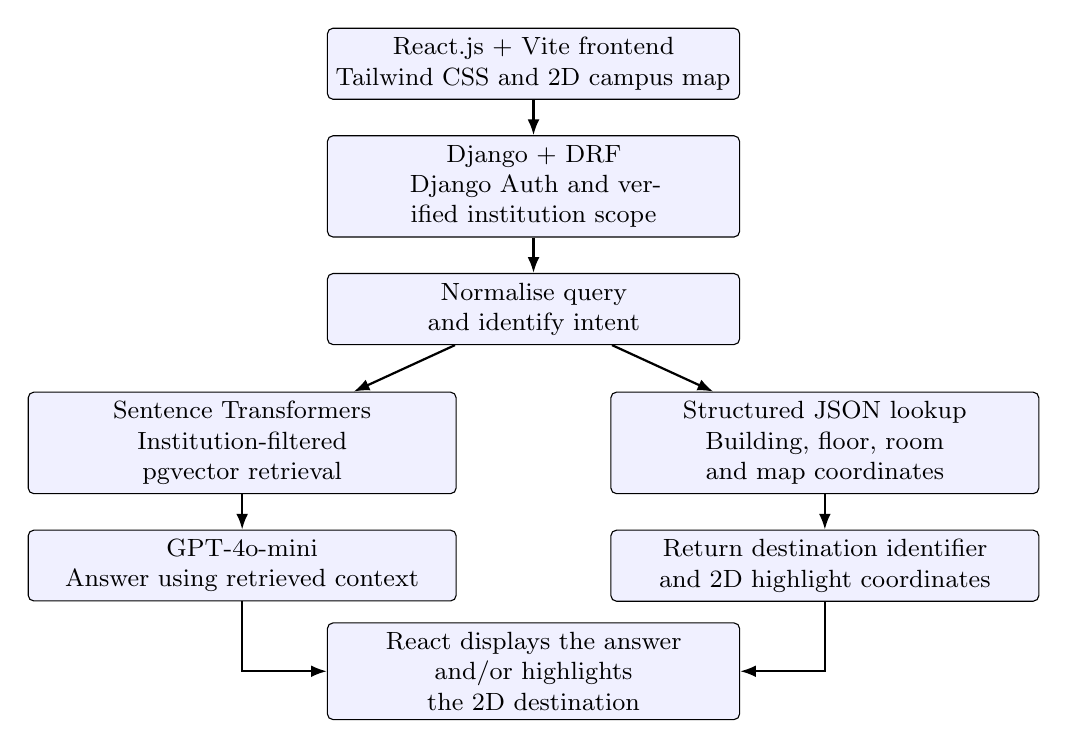
\begin{tikzpicture}[node distance=0.45cm]
  \node[process,text width=5cm] (frontend) {React.js + Vite frontend\\Tailwind CSS and 2D campus map};
  \node[process,text width=5cm,below=of frontend] (auth) {Django + DRF\\Django Auth and verified institution scope};
  \node[process,text width=5cm,below=of auth] (intent) {Normalise query and identify intent};
  \node[process,text width=5.2cm] (retrieval) at ($(intent.center)+(-3.7,-1.7)$)
    {Sentence Transformers\\Institution-filtered pgvector retrieval};
  \node[process,text width=5.2cm] (location) at ($(intent.center)+(3.7,-1.7)$)
    {Structured JSON lookup\\Building, floor, room and map coordinates};
  \node[process,text width=5.2cm,below=of retrieval] (generation)
    {GPT-4o-mini\\Answer using retrieved context};
  \node[process,text width=5.2cm,below=of location] (map)
    {Return destination identifier\\and 2D highlight coordinates};
  \node[process,text width=5cm] (response) at ($(intent.center)+(0,-4.6)$)
    {React displays the answer\\and/or highlights the 2D destination};
  \draw[flow] (frontend) -- (auth);
  \draw[flow] (auth) -- (intent);
  \draw[flow] (intent) -- (retrieval);
  \draw[flow] (intent) -- (location);
  \draw[flow] (retrieval) -- (generation);
  \draw[flow] (location) -- (map);
  \draw[flow] (generation.south) |- (response.west);
  \draw[flow] (map.south) |- (response.east);
\end{tikzpicture}
\caption{v1 request architecture: Django/DRF, institution-scoped RAG and 2D navigation.}
\label{fig:high-level-flow}
\end{figure}

\subsection{Technical Stack}

Table~\ref{tab:stack} records the project-specific technology choices. A v1
classification identifies the initial technical baseline, not evidence that
a deployment or performance target has already been validated.

\begin{table}[htbp]
\centering
\small
\renewcommand{\arraystretch}{1.15}
\begin{tabularx}{\linewidth}{@{}>{\raggedright\arraybackslash}p{2.65cm}>{\raggedright\arraybackslash}p{3.65cm}Y@{}}
\toprule
\textbf{Component} & \textbf{Technology} & \textbf{Responsibility and scope} \\
\midrule
Web interface & React.js, Vite, Tailwind CSS & Student/admin screens and UI styling (v1). \\
Backend API & Python, Django, DRF & Authentication, domain logic and REST endpoints (v1). \\
Relational storage & PostgreSQL & Institutions, students, faculty, courses, events, notices and document metadata (v1). \\
Vector retrieval & pgvector & Store chunk embeddings and perform institution-scoped similarity search (v1). \\
Embedding model & Sentence Transformers & Embed document chunks and student queries (v1). \\
Answer generation & GPT-4o-mini & Generate responses from retrieved context through a custom Python RAG pipeline (v1). \\
Document ingestion & PyMuPDF & Extract text from institutional PDF documents before chunking and embedding (v1). \\
Access control & Django Auth; institutional email check & Authenticate users, verify affiliation and authorise institution-scoped access (v1). \\
Administration & Django Admin & Maintain institutional records and approved knowledge documents (v1). \\
Campus navigation & SVG / floor-plan images; structured JSON & Resolve and highlight buildings, floors and rooms on a 2D map (v1). \\
Testing and delivery & pytest, Postman, Git, GitHub & Unit/API tests, version control and automated build/test workflow (v1). \\
Hosting targets & Vercel; Render / Railway & Frontend hosting, backend staging and PostgreSQL with pgvector support (v1 targets). \\
3D extension & Three.js, Blender & Interactive 3D scenes and campus assets (roadmap). \\
\bottomrule
\end{tabularx}
\caption{Technical baseline and roadmap aligned with the project report.}
\label{tab:stack}
\end{table}

\subsection{UML Design Views}

Unified Modeling Language (UML) is used here to describe complementary aspects
of the design: the use case diagram identifies user interactions, the class
diagram models domain structure, the activity diagram describes control flow,
and the sequence diagram specifies message ordering. These diagrams describe
the intended design; they are not reverse-engineered evidence of completed code.
The SDLC diagram separately documents the development process.

\subsection{Use Case Diagram}

Students authenticate and verify institutional affiliation before submitting
questions or viewing campus locations. Academic and event questions use the
same grounded-query workflow. College administrators maintain approved
knowledge, institutional records and location mappings through authorised
administrative interfaces. Personal reminders are a later extension and are
shown separately as roadmap scope.

\begin{figure}[htbp]
\centering
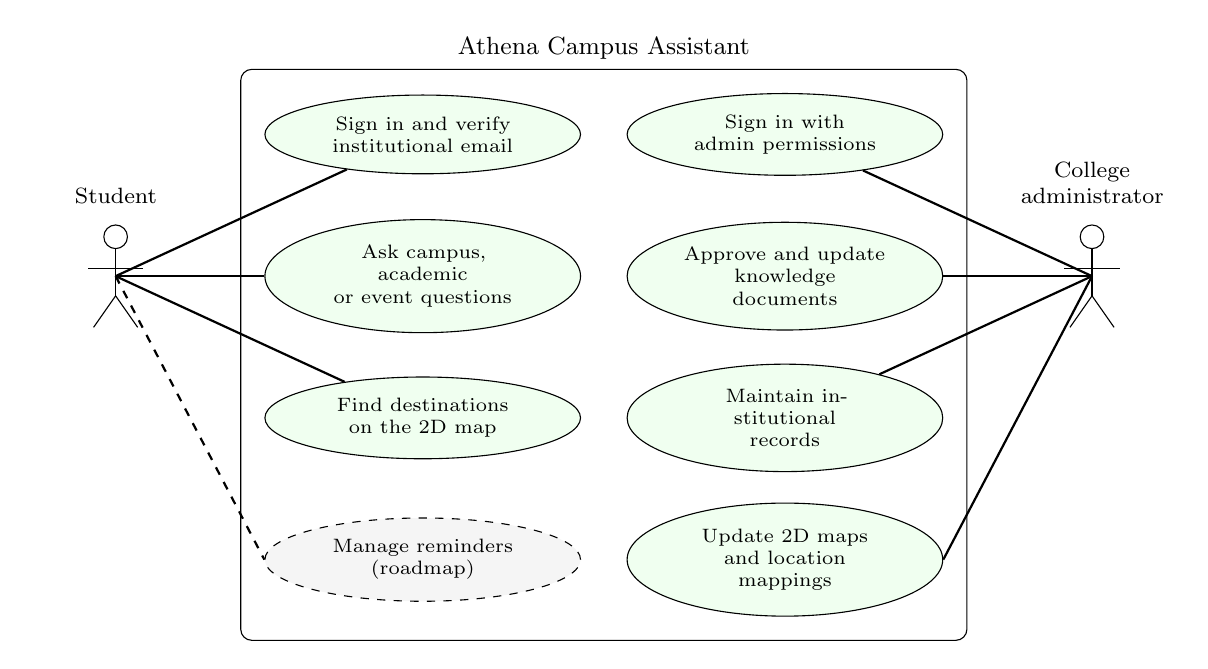
\begin{tikzpicture}[
  actor/.style={align=center,font=\footnotesize,text width=2cm},
  usecase/.style={ellipse,draw,fill=green!6,text width=2.6cm,
    minimum height=1cm,align=center,font=\scriptsize}
]
  \coordinate (student) at (-6.2,-1.8);
  \coordinate (admin) at (6.2,-1.8);
  \foreach \actorname in {student,admin} {
    \draw ($(\actorname)+(0,0.5)$) circle (0.15cm);
    \draw ($(\actorname)+(0,0.35)$) -- ($(\actorname)+(0,-0.25)$);
    \draw ($(\actorname)+(-0.35,0.1)$) -- ($(\actorname)+(0.35,0.1)$);
    \draw ($(\actorname)+(-0.28,-0.65)$) -- ($(\actorname)+(0,-0.25)$)
      -- ($(\actorname)+(0.28,-0.65)$);
  }
  \node[actor,above=0.8cm of student] {Student};
  \node[actor,above=0.8cm of admin] {College\\administrator};
  \node[usecase] (verify) at (-2.3,0) {Sign in and verify\\institutional email};
  \node[usecase] (ask) at (-2.3,-1.8) {Ask campus, academic\\or event questions};
  \node[usecase] (navigate) at (-2.3,-3.6) {Find destinations\\on the 2D map};
  \node[usecase,dashed,fill=gray!8] (reminders) at (-2.3,-5.4) {Manage reminders\\(roadmap)};
  \node[usecase] (adminlogin) at (2.3,0) {Sign in with\\admin permissions};
  \node[usecase] (documents) at (2.3,-1.8) {Approve and update\\knowledge documents};
  \node[usecase] (records) at (2.3,-3.6) {Maintain institutional\\records};
  \node[usecase] (locations) at (2.3,-5.4) {Update 2D maps\\and location mappings};
  \begin{scope}[on background layer]
    \node[draw,rounded corners,inner sep=0.3cm,
      fit=(verify)(ask)(navigate)(reminders)(adminlogin)(documents)(records)(locations),
      label={[font=\small]above:Athena Campus Assistant}] {};
  \end{scope}
  \draw[association] (student) -- (verify);
  \draw[association] (student) -- (ask);
  \draw[association] (student) -- (navigate);
  \draw[association,dashed] (student) -- (reminders.west);
  \draw[association] (admin) -- (adminlogin);
  \draw[association] (admin) -- (documents);
  \draw[association] (admin) -- (records);
  \draw[association] (admin) -- (locations.east);
\end{tikzpicture}
\caption{UML use case view. Protected actions require verified affiliation or administrative permissions; dashed scope is planned.}
\label{fig:usecase}
\end{figure}

\subsection{Class Diagram}

Figure~\ref{fig:class} models the principal institutional entities together
with application-level behaviours. Student and administrator accounts use
Django Auth; a profile or membership links an account to its institution.
Knowledge documents supply chunks for retrieval, courses are associated with
faculty, and societies organise events. The Reminder class is a roadmap
extension. Operations shown are design responsibilities, not claims about
exact method names in an existing implementation.

\begin{figure}[htbp]
\centering
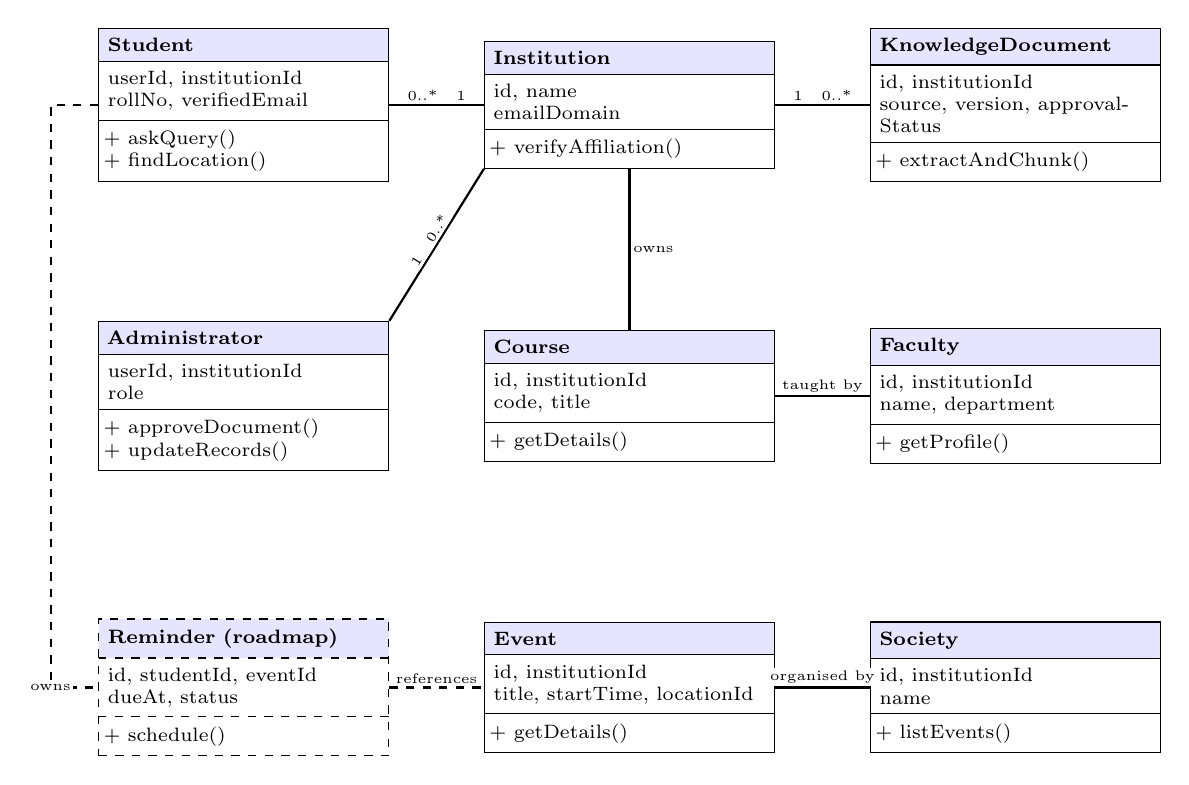
\begin{tikzpicture}[
  cls/.style={rectangle split,rectangle split parts=3,draw,
    align=left,font=\scriptsize,text width=3.45cm,
    rectangle split part fill={blue!10,white,white}},
  relationlabel/.style={font=\tiny,fill=white,inner sep=1pt}
]
  \node[cls] (student) at (-4.9,0) {\textbf{Student}
    \nodepart{second} userId, institutionId\\rollNo, verifiedEmail
    \nodepart{third} + askQuery()\\+ findLocation()};
  \node[cls] (institution) at (0,0) {\textbf{Institution}
    \nodepart{second} id, name\\emailDomain
    \nodepart{third} + verifyAffiliation()};
  \node[cls] (document) at (4.9,0) {\textbf{KnowledgeDocument}
    \nodepart{second} id, institutionId\\source, version, approvalStatus
    \nodepart{third} + extractAndChunk()};
  \node[cls] (admin) at (-4.9,-3.7) {\textbf{Administrator}
    \nodepart{second} userId, institutionId\\role
    \nodepart{third} + approveDocument()\\+ updateRecords()};
  \node[cls] (course) at (0,-3.7) {\textbf{Course}
    \nodepart{second} id, institutionId\\code, title
    \nodepart{third} + getDetails()};
  \node[cls] (faculty) at (4.9,-3.7) {\textbf{Faculty}
    \nodepart{second} id, institutionId\\name, department
    \nodepart{third} + getProfile()};
  \node[cls,dashed] (reminder) at (-4.9,-7.4) {\textbf{Reminder (roadmap)}
    \nodepart{second} id, studentId, eventId\\dueAt, status
    \nodepart{third} + schedule()};
  \node[cls] (event) at (0,-7.4) {\textbf{Event}
    \nodepart{second} id, institutionId\\title, startTime, locationId
    \nodepart{third} + getDetails()};
  \node[cls] (society) at (4.9,-7.4) {\textbf{Society}
    \nodepart{second} id, institutionId\\name
    \nodepart{third} + listEvents()};
  \draw[association] (student) -- node[relationlabel,above] {0..*\quad 1} (institution);
  \draw[association] (institution) -- node[relationlabel,above] {1\quad 0..*} (document);
  \draw[association] (institution.south west) -- node[relationlabel,sloped,above] {1\quad 0..*} (admin.north east);
  \draw[association] (institution) -- node[relationlabel,right] {owns} (course);
  \draw[association] (course) -- node[relationlabel,above] {taught by} (faculty);
  \draw[association] (event) -- node[relationlabel,above] {organised by} (society);
  \draw[association,dashed] (reminder) -- node[relationlabel,above] {references} (event);
  \draw[association,dashed] (student.west) -- ++(-0.6,0)
    |- node[relationlabel,pos=0.75,left] {owns} (reminder.west);
\end{tikzpicture}
\caption{UML class model for institutional knowledge and campus services; the dashed reminder extension is outside v1.}
\label{fig:class}
\end{figure}

Institution identifiers scope faculty, courses, events and societies as well
as documents and accounts. Only selected associations are drawn to keep the
model legible. Each knowledge document may produce multiple chunks; pgvector
stores the corresponding embeddings with links to the document and institution.
This is distinct from assigning one embedding to an entire document.

For navigation, the v1 report specifies structured JSON rather than a separate
relational building/floor/room schema. The proposed location contract comprises
\texttt{institutionId}, \texttt{locationId}, \texttt{building}, \texttt{floor},
\texttt{room}, \texttt{mapId} and 2D coordinates. Campus identifiers must remain
consistent across event records, JSON mappings and SVG or floor-plan assets.

\subsection{Activity Diagram}

Figure~\ref{fig:activity} shows the primary flow for a single-intent query.
Unauthorised requests terminate before retrieval or location lookup. The two
successful processing branches converge only after their respective results
have been prepared. Ambiguous locations and insufficient document evidence
should produce clarification or an explicit inability to answer, rather than
an unsupported destination or response.

\begin{figure}[htbp]
\centering
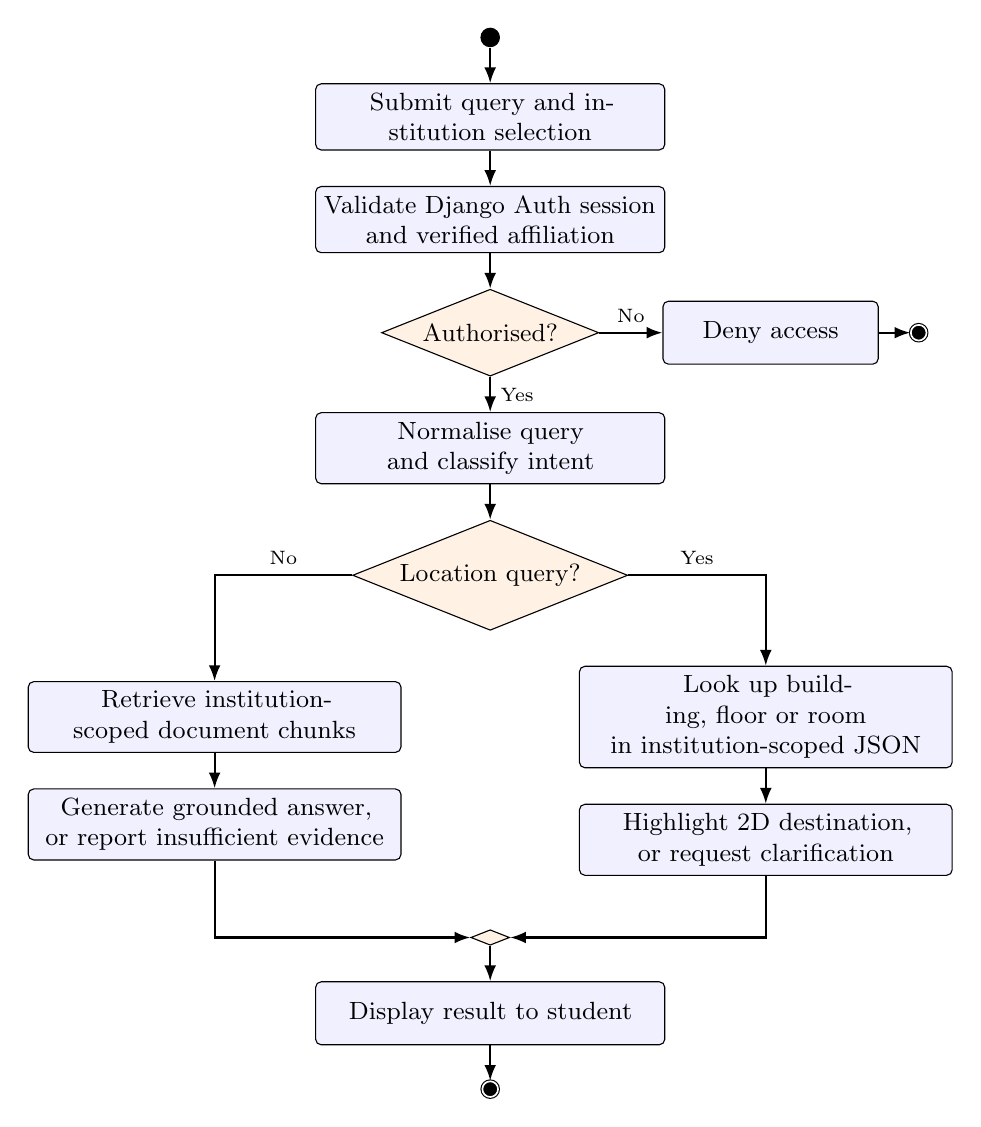
\begin{tikzpicture}[node distance=0.45cm]
  \node[circle,fill=black,inner sep=2.5pt] (start) {};
  \node[process,below=of start] (input) {Submit query and institution selection};
  \node[process,below=of input] (auth) {Validate Django Auth session\\and verified affiliation};
  \node[decision,below=of auth] (allowed) {Authorised?};
  \node[process,text width=2.5cm,right=0.8cm of allowed] (reject) {Deny access};
  \node[circle,draw,double,fill=black,inner sep=2pt,right=0.4cm of reject] (denied) {};
  \node[process,below=of allowed] (nlp) {Normalise query and classify intent};
  \node[decision,below=of nlp] (intent) {Location query?};
  \node[process,text width=4.5cm] (rag) at ($(intent.center)+(-3.5,-1.8)$)
    {Retrieve institution-scoped document chunks};
  \node[process,text width=4.5cm] (resolve) at ($(intent.center)+(3.5,-1.8)$)
    {Look up building, floor or room\\in institution-scoped JSON};
  \node[process,text width=4.5cm,below=of rag] (answer)
    {Generate grounded answer, or report insufficient evidence};
  \node[process,text width=4.5cm,below=of resolve] (render)
    {Highlight 2D destination,\\or request clarification};
  \node[decision] (merge) at ($(intent.center)+(0,-4.6)$) {};
  \node[process,below=of merge] (display) {Display result to student};
  \node[circle,draw,double,fill=black,inner sep=2pt,below=of display] (end) {};
  \draw[flow] (start) -- (input);
  \draw[flow] (input) -- (auth);
  \draw[flow] (auth) -- (allowed);
  \draw[flow] (allowed) -- node[above,font=\scriptsize] {No} (reject);
  \draw[flow] (reject) -- (denied);
  \draw[flow] (allowed) -- node[right,font=\scriptsize] {Yes} (nlp);
  \draw[flow] (nlp) -- (intent);
  \draw[flow] (intent.west) -| node[above,pos=0.25,font=\scriptsize] {No} (rag.north);
  \draw[flow] (intent.east) -| node[above,pos=0.25,font=\scriptsize] {Yes} (resolve.north);
  \draw[flow] (rag) -- (answer);
  \draw[flow] (resolve) -- (render);
  \draw[flow] (answer.south) |- (merge.west);
  \draw[flow] (render.south) |- (merge.east);
  \draw[flow] (merge) -- (display);
  \draw[flow] (display) -- (end);
\end{tikzpicture}
\caption{Student-query activity flow, including access denial and convergence of the result paths.}
\label{fig:activity}
\end{figure}

\subsection{UML Sequence Diagram}

Figure~\ref{fig:sequence} shows the message order for an authorised knowledge
query with sufficient retrieved evidence. Authentication and affiliation checks
precede retrieval. The location-only path uses JSON lookup instead of an LLM
call; access-denied and insufficient-evidence outcomes are handled by the
activity flow and the safeguards described below.

\begin{figure}[htbp]
\centering
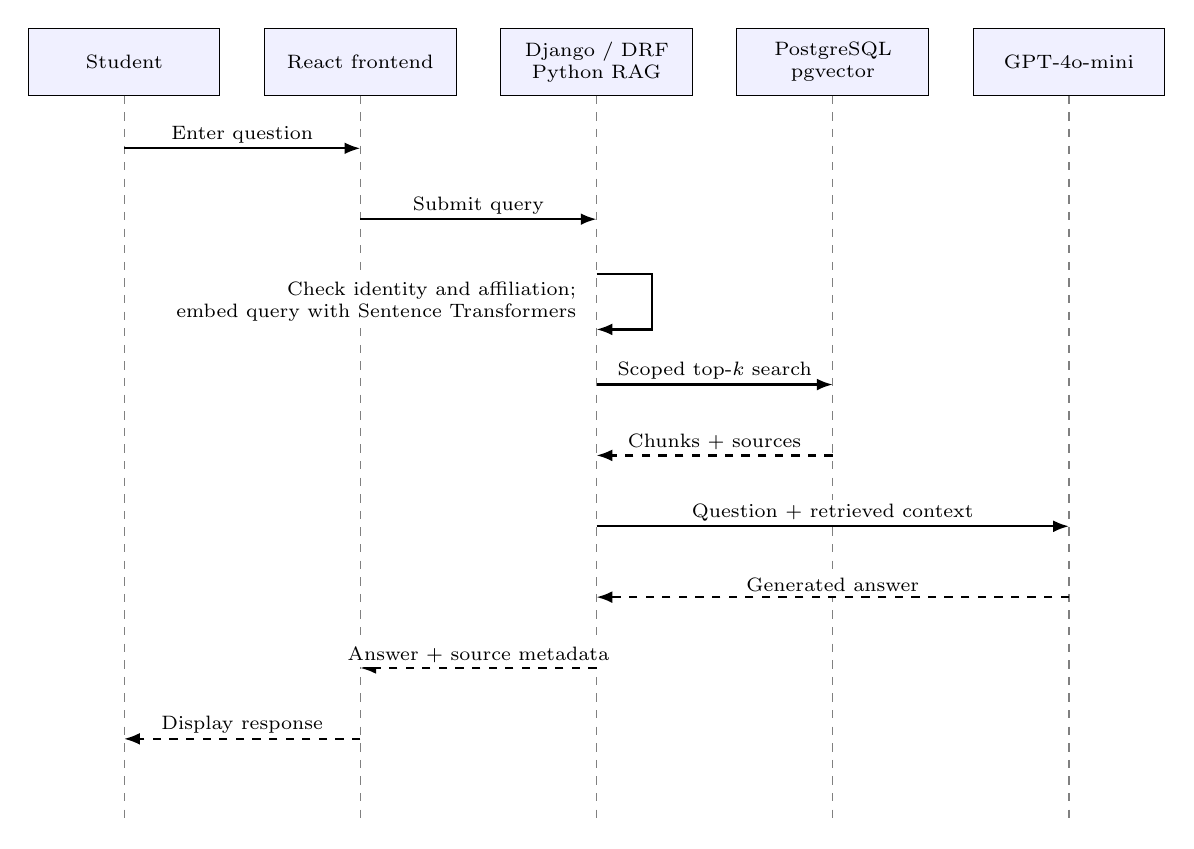
\begin{tikzpicture}[
  participant/.style={draw,fill=blue!6,text width=2.2cm,minimum height=0.85cm,
    align=center,font=\scriptsize},
  message/.style={font=\scriptsize,fill=white,inner sep=1.5pt},
  reply/.style={flow,dashed}
]
  \node[participant] (student) at (0,0) {Student};
  \node[participant] (react) at (3,0) {React frontend};
  \node[participant] (django) at (6,0) {Django / DRF\\Python RAG};
  \node[participant] (vector) at (9,0) {PostgreSQL\\pgvector};
  \node[participant] (llm) at (12,0) {GPT-4o-mini};
  \foreach \participantname in {student,react,django,vector,llm}
    \draw[dashed,gray] (\participantname.south) -- ++(0,-9.2);
  \draw[flow] (0,-1.1) -- node[message,above] {Enter question} (3,-1.1);
  \draw[flow] (3,-2) -- node[message,above] {Submit query} (6,-2);
  \draw[flow] (6,-2.7) -- (6.7,-2.7) -- (6.7,-3.4) -- (6,-3.4);
  \node[message,anchor=east,align=right] at (5.8,-3.05)
    {Check identity and affiliation;\\embed query with Sentence Transformers};
  \draw[flow] (6,-4.1) -- node[message,above] {Scoped top-$k$ search} (9,-4.1);
  \draw[reply] (9,-5) -- node[message,above] {Chunks + sources} (6,-5);
  \draw[flow] (6,-5.9) -- node[message,above] {Question + retrieved context} (12,-5.9);
  \draw[reply] (12,-6.8) -- node[message,above] {Generated answer} (6,-6.8);
  \draw[reply] (6,-7.7) -- node[message,above] {Answer + source metadata} (3,-7.7);
  \draw[reply] (3,-8.6) -- node[message,above] {Display response} (0,-8.6);
\end{tikzpicture}
\caption{UML sequence diagram for the successful v1 RAG query workflow.}
\label{fig:sequence}
\end{figure}

\subsection{Implementation Details}

\paragraph{Module 1: document ingestion and knowledge maintenance.}
An authorised administrator uploads or updates an approved institutional
PDF through the administrative workflow. PyMuPDF extracts text, which the
custom Python pipeline normalises and splits into retrievable chunks.
Sentence Transformers generates chunk embeddings for storage through pgvector.
Document identifiers, source metadata and institution identifiers must be
retained so retrieved passages remain attributable and correctly scoped.
Document updates should replace or retire obsolete chunks rather than leaving
contradictory versions active. Chunk size, overlap and the exact embedding
model configuration must be recorded for evaluation; the project report does
not fix these values.

\paragraph{Module 2: retrieval-grounded query answering.}
The DRF endpoint invokes the custom Python RAG pipeline after authorisation.
The query is embedded using a configuration compatible with stored chunks,
and institution-filtered similarity search returns the top-$k$ passages from
pgvector. GPT-4o-mini receives the question and retrieved evidence, not the
raw question alone. The response should retain source metadata for inspection.
If evidence is absent or inadequate, the application should return an explicit
insufficient-information response instead of presenting an unsupported answer.
Retrieval and prompting do not guarantee correctness; answer grounding and
relevance require separate evaluation.

\paragraph{Module 3: authentication and institutional verification.}
Django Auth supplies the account-authentication layer. The v1 affiliation
mechanism is an institutional-email check associated with the user's
authenticated account. The security requirement is to
confirm ownership of an approved institutional email address before enabling
protected access; a domain string supplied by the client is not sufficient.
The report does not specify the email-confirmation implementation, so this
remains a validation requirement. Backend authorisation must enforce the
verified institution and role on every protected operation. Django Admin
permissions restrict document and institutional-record maintenance.

\paragraph{Module 4: 2D campus navigation.}
The React interface displays SVG campus maps or floor-plan images. Location
queries resolve to structured JSON entries describing the building, floor,
room, map asset and highlight coordinates. Unknown destinations should return
a not-found response; ambiguous names should trigger clarification. Three.js
rendering, Blender assets and turn-by-turn directions are roadmap work, not
part of the v1 navigation claim.

\paragraph{Module 5: academic information and future personalisation.}
Institution-scoped course, faculty, event, society and notice records support
campus-information queries and administrative maintenance. Personalised
student dashboards and date reminders are subsequent deliverables; the class
and use case diagrams mark them as planned rather than implemented.

\subsection{Deployment and CI/CD}

The frontend deployment target is Vercel; the Django/DRF backend target is
Render or Railway, with PostgreSQL configured to support pgvector. The
backend, not the browser, communicates with the external language-model API.
Model credentials and database connection settings belong in deployment
configuration, not frontend bundles or committed source files.

The planned CI/CD workflow builds the React application and runs backend unit
tests on code changes, then produces a repeatable staging release. Postman
workflows validate login, affiliation, querying and map lookup after deployment.
Git and GitHub provide version control and collaboration; the exact runner
configuration and production release policy still need to be documented.

\begin{figure}[htbp]
\centering
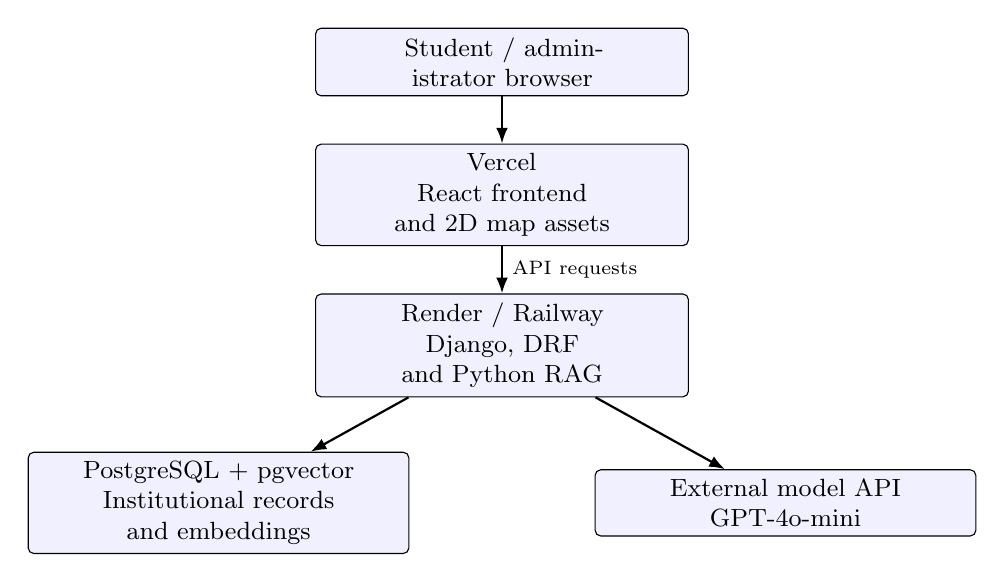
\begin{tikzpicture}[node distance=0.6cm]
  \node[process,text width=4.5cm] (browser) {Student / administrator browser};
  \node[process,text width=4.5cm,below=of browser] (vercel) {Vercel\\React frontend and 2D map assets};
  \node[process,text width=4.5cm,below=of vercel] (backend) {Render / Railway\\Django, DRF and Python RAG};
  \node[process,text width=4.6cm] (database) at ($(backend.center)+(-3.6,-2)$)
    {PostgreSQL + pgvector\\Institutional records and embeddings};
  \node[process,text width=4.6cm] (openai) at ($(backend.center)+(3.6,-2)$)
    {External model API\\GPT-4o-mini};
  \draw[flow] (browser) -- (vercel);
  \draw[flow] (vercel) -- node[right,font=\scriptsize] {API requests} (backend);
  \draw[flow] (backend) -- (database);
  \draw[flow] (backend) -- (openai);
\end{tikzpicture}
\caption{Planned deployment responsibilities. Hosting targets do not imply a verified live deployment.}
\label{fig:deployment}
\end{figure}

\section{Software Development Life Cycle}

Athena follows an \textbf{Agile, iterative} SDLC organised around weekly
increments and rapid feedback. The first release prioritises a single-college
query workflow over a broad but incomplete feature set. Each iteration refines
requirements, updates the design, implements changes, executes automated checks
and releases an increment to staging for review.

\begin{figure}[htbp]
\centering
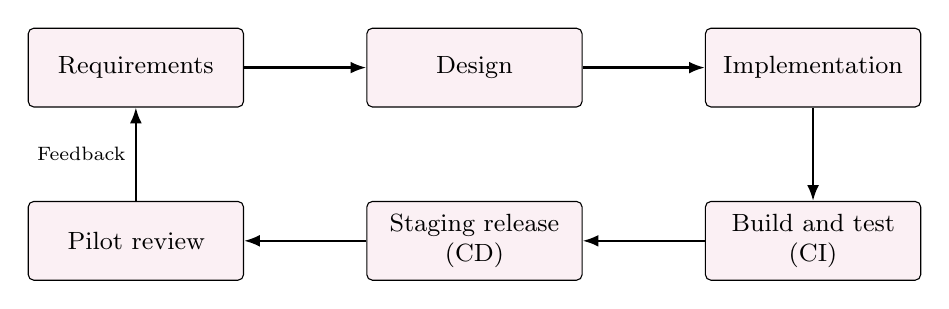
\begin{tikzpicture}[
  phase/.style={process,text width=2.5cm,minimum height=1cm,fill=purple!6}
]
  \node[phase] (requirements) at (0,0) {Requirements};
  \node[phase] (design) at (4.3,0) {Design};
  \node[phase] (implementation) at (8.6,0) {Implementation};
  \node[phase] (testing) at (8.6,-2.2) {Build and test\\(CI)};
  \node[phase] (deployment) at (4.3,-2.2) {Staging release\\(CD)};
  \node[phase] (review) at (0,-2.2) {Pilot review};
  \draw[flow] (requirements) -- (design);
  \draw[flow] (design) -- (implementation);
  \draw[flow] (implementation) -- (testing);
  \draw[flow] (testing) -- (deployment);
  \draw[flow] (deployment) -- (review);
  \draw[flow] (review) -- node[left,font=\scriptsize] {Feedback} (requirements);
\end{tikzpicture}
\caption{Weekly iterative SDLC with continuous integration, staging delivery and pilot feedback.}
\label{fig:sdlc}
\end{figure}

The proposed increment order is:
\begin{enumerate}
  \item \textbf{Core information workflow:} establish React and Django/DRF,
    institution records, document ingestion and pgvector-backed answering.
  \item \textbf{Verified pilot and navigation:} complete institutional-email
    verification, administrative maintenance and 2D location highlighting;
    exercise the workflow with one college and collect evaluation evidence.
  \item \textbf{Expansion after validation:} improve answer quality and staging
    reliability, then extend institution coverage and introduce roadmap
    features such as reminders and interactive 3D navigation.
\end{enumerate}

Each increment should have explicit acceptance checks: correct API behaviour,
rejection of unauthorised cross-institution requests, source-supported answers,
and correct mapped destinations. Sprint numbering and completion dates should
be recorded from actual development logs rather than inferred from this plan.

\chapter{Results and Evaluation}
\label{chap:evaluation}

\section{Testing Methodology}

The evaluation separates component correctness, end-to-end behaviour,
institution isolation and user-facing quality. The project uses pytest and
Postman as its principal test tools; quantitative outcomes remain pending until
execution logs, dataset sizes and measured values are documented.

\begin{itemize}
  \item \textbf{Unit testing:} test query normalisation, retrieval-filter
    construction, affiliation checks and location lookup independently.
    External model services should be mocked where deterministic assertions
    are required.
  \item \textbf{Integration testing:} exercise authentication, query submission,
    context retrieval, answer delivery and location highlighting as connected
    workflows. Verify behaviour for empty retrieval results, unknown rooms,
    ambiguous names and service failures.
  \item \textbf{Isolation and authorisation testing:} use at least two test
    institutions and attempt cross-institution document and location access.
    Include invalid or expired sessions, unverified email addresses, modified institution
    identifiers and administrative actions attempted with student privileges.
  \item \textbf{Performance testing:} measure end-to-end query latency under
    a documented workload. Record model configuration, corpus size, value of
    $k$, hardware, network conditions, cache state and concurrency so that
    measurements can be interpreted and reproduced.
  \item \textbf{Pilot user evaluation:} recruit students and an administrator
    from one institution. Log query outcomes and collect direct feedback on
    answer relevance and destination-finding task completion. Compare outcomes
    across documented iterations; participant counts and results remain pending.
\end{itemize}

\section{Performance Metrics}

The primary evaluation criterion is \textbf{answer groundedness and relevance}:
whether an answer is supported by retrieved institutional evidence and useful
to the student asking the question. Grounding and student-rated relevance
should be reported separately as well as jointly. Secondary metrics cover
latency, location resolution, legitimate-student verification and service
availability during the declared pilot operating window.

The project report does not supply measured results or fixed numerical
acceptance thresholds. These must be established before the pilot and then
reported with the test-set size, workload and configuration. Table~\ref{tab:performance}
therefore states criteria without presenting proposed targets as achieved values.

\begin{table}[htbp]
\centering
\small
\renewcommand{\arraystretch}{1.2}
\begin{tabularx}{\linewidth}{@{}Y Y Y@{}}
\toprule
\textbf{Metric} & \textbf{Evaluation criterion} & \textbf{Evidence status} \\
\midrule
Answer grounding & Factual claims supported by retrieved sources & Source-based review pending \\
Student-rated relevance & Response addresses the student's information need & Pilot feedback pending \\
Joint answer success & Answer is both grounded and judged relevant & Curated-query evaluation pending \\
Retrieval precision at $k$ & Relevant chunks among the retrieved top-$k$ & Labelled retrieval test pending \\
Query response time & Submission-to-display latency; report median and 95th percentile & Timing measurements pending \\
Verification success rate & Legitimate students correctly verified & Positive and negative tests pending \\
Institution isolation & No successful unauthorised access in the test suite & Adversarial access tests pending \\
2D navigation accuracy & Correct building, floor or room highlighted & Annotated location tests pending \\
Service reliability & Login and query availability during declared pilot hours & Staging monitoring pending \\
\bottomrule
\end{tabularx}
\caption{Evaluation criteria for the v1 pilot. All quantitative outcomes await documented measurement.}
\label{tab:performance}
\end{table}

For a labelled set of $N$ knowledge queries, retrieval precision is defined as
\[
  P@k = \frac{1}{N}\sum_{i=1}^{N}
    \frac{\text{number of relevant chunks among the top }k\text{ for query }i}{k}.
\]
Fix $k$ and the relevance criteria before testing. If fewer than $k$ chunks are
returned, missing positions count as non-relevant for this metric. Retrieval
precision does not measure whether the generated answer is correct or complete.

The \emph{answer grounding rate} is the proportion of substantive answers for
which every factual claim is supported by the retrieved institutional evidence.
Abstentions are reported separately, together with the proportion of queries
receiving a substantive answer, to avoid treating non-answers as successful
grounding. Verification success is the proportion of legitimate test users
correctly verified. False acceptances among unauthorised users and false
rejections among legitimate users should also be reported separately. Perfect performance on a finite suite does not prove
security for all possible requests.

Location resolution accuracy is the proportion of annotated, unambiguous,
in-scope queries mapped to the correct destination identifier. Unknown or
ambiguous destinations should be evaluated separately for appropriate refusal
or clarification. Coverage is reported as mapped locations divided by the total
locations in a declared campus inventory, with building and room counts stated
explicitly.

\section{Prototype Status and Analysis}

The project report specifies the v1 stack and initial deliverables: React and
Tailwind screens, Django/DRF endpoints, Django Auth and institutional-email
verification, document ingestion, pgvector retrieval, GPT-4o-mini answering,
2D navigation and CI/CD to staging. These define the technical baseline for
Objectives~1--4. They are not accompanied by execution logs, deployment checks
or quantitative pilot results, so this report does not claim that the
acceptance criteria have already been met.

The central integration challenge is to connect ingestion, verified access and
retrieval without losing institution scope or source attribution. A separate
navigation challenge is to keep location identifiers and 2D map coordinates
consistent with campus records. Source refresh, reliable query handling and
correct highlighting should be validated before expanding to multiple colleges
or introducing 3D assets.

\section{Limitations and Threats to Validity}

The principal limitation is the absence of reported quantitative results and
reproducible test artefacts. A small or unrepresentative query set could
overestimate answer quality; outdated or incomplete documents could yield
answers that are grounded in their sources but no longer correct for students.
Knowledge-base approval therefore needs document maintenance and version tracking.

The exact Sentence Transformers model, chunking parameters, retrieval settings,
email-verification workflow and deployment configuration remain to be documented.
External-model variation and network conditions may affect answer quality and
latency. A single-college pilot and limited map coverage cannot establish
performance or usability across all institutions. Final evaluation should state
the number of documents, queries, mapped locations, institutions and participants,
and specify how long staging availability was monitored.

\chapter{Conclusion}

\section{Summary of Work}

Athena is designed as a web-based campus companion combining verified
institutional knowledge with conversational access and location search. Its
v1 baseline uses React.js, Vite and Tailwind CSS; Django and DRF; PostgreSQL
with pgvector; Sentence Transformers; PyMuPDF; and GPT-4o-mini. Django Auth,
institutional-email verification and Django Admin support access and maintenance.
Navigation initially uses 2D maps and structured JSON, while Three.js and Blender
remain part of the roadmap.

The engineering contribution is the integration of mature components into a
measurable, deployable workflow, rather than a claim of novel retrieval
algorithms. The use case, class, activity and sequence diagrams describe the
system design; the deployment and SDLC views connect that design to incremental
delivery. Actual performance remains to be established through a documented pilot.

\section{Key Findings}

\begin{itemize}
  \item \textbf{Institution scope must be enforced throughout the backend.}
    Authentication, affiliation checks, document retrieval, JSON location lookup
    and administrative operations must share the same authorised institution
    context; prompt instructions are not an access-control mechanism.
  \item \textbf{Grounding and usefulness are different requirements.} Source
    support must be assessed alongside the student's judgement of relevance,
    with insufficient-evidence cases recorded explicitly.
  \item \textbf{A 2D-first release limits initial integration scope.} SVG or
    floor-plan maps and structured location records provide a testable navigation
    workflow before investment in 3D assets and routing.
  \item \textbf{Fast feedback needs repeatable delivery.} Automated builds,
    backend tests and staging releases support short iterations whose changes
    can be evaluated against a consistent pilot workflow.
\end{itemize}

These are design conclusions and evaluation priorities, not quantitative
experimental findings.

\section{Future Work and Recommendations}

\begin{enumerate}
  \item \textbf{Validate the first-college pilot.} Define acceptance thresholds,
    assemble labelled queries, test email verification and institution isolation,
    and report groundedness, relevance, latency, navigation accuracy and uptime.
  \item \textbf{Extend navigation after v1.} Expand the 2D location inventory,
    then add Three.js scenes and Blender-authored models. Turn-by-turn directions
    require a connected routing representation in addition to destination coordinates.
  \item \textbf{Improve knowledge and multi-college administration.} Strengthen
    approval, versioning and refresh workflows, and develop the planned admin
    dashboard for maintaining multiple independently scoped institutions.
  \item \textbf{Add personalised services.} Introduce student dashboards and
    academic or campus-date reminders after the core query workflow is evaluated.
  \item \textbf{Broaden interaction and integration.} Explore voice assistance,
    mobile access, ERP and attendance integration, and personalised academic help.
  \item \textbf{Harden delivery.} Document Vercel and Render/Railway staging,
    database migrations, secret management, monitoring and rollback procedures
    before claiming production reliability or scalability.
\end{enumerate}

\section{Final Remarks}

Athena addresses fragmented campus information through verified access,
retrieval-grounded answers and a searchable campus map. A single-college,
2D-first pilot provides a focused starting point, while institution-scoped
records and modular web components allow later expansion. The next priority
is evidence: documented tests and student feedback should guide each release
before broader deployment and roadmap features are introduced.

\printbibliography[heading=bibintoc]
\end{document}
